\chapter{User Manual}

\startcontents[chapters]
\printcontents[chapters]{}{1}{}

\section{Introduction}
\subsection{purpose}
The purpose of the system is to provide an easy to use metering solution for several types of consumption which the user can specify with each type allowing for many readings to be stored at any time. It is also meant to allow for the data that is stored to be called upon at any time to be displayed in a wide range of visual outputs such as graphs and tables.

This is achieved through several features such as:
\begin{itemize}
	\item Creation of types - Consumption types can be created, edited and removed and each one can have individual names and descriptions.
	\item Reading and Cost input windows - Readings and their costs can be added, edited or removed through easy to use windows with labels by their corresponding input boxes.
	\item Visual output of data inside the database - Data is displayed in a range of visual outputs such as bar charts, pie charts and tables.
\end{itemize}

\subsection{Intended audience}
The intended audience for the system was Michael Seamark. However, it can be used by other companies or people without too much change being required if they need this system.

\section{Installation}

\subsection{Prerequisite Installation}
\label{Prerequisite_Installation}

%include as many subsubsections as necessary for each piece of required software
\subsubsection{Installing Python}
\begin{enumerate}
	\item go to https://www.python.org
	\item click the downloads button
	\item click python 3.4.3
\begin{figure}[H]
	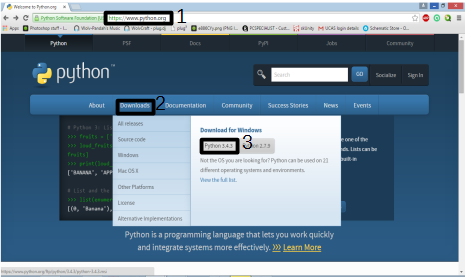
\includegraphics{./manual/images/python-installation-instructions-1.png}
	\caption{How to install python steps 1, 2 and 3}
\end{figure}

	\item navigate to the location the installer was saved to and open it
	
\begin{figure}[H]
	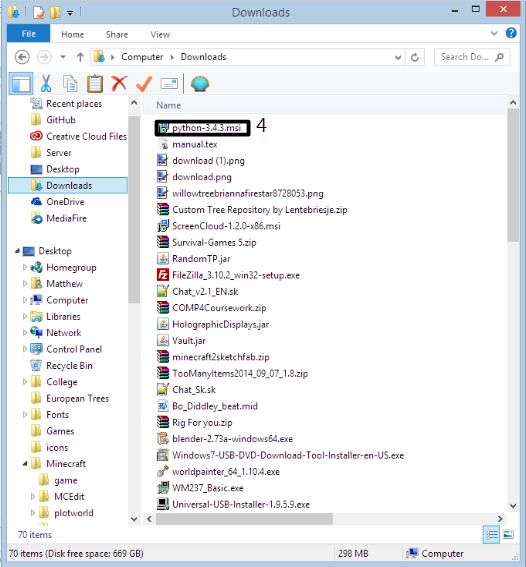
\includegraphics{./manual/images/python-installation-instructions-2.png}
	\caption{How to install python step 4}
\end {figure}

\begin{figure}[H]
	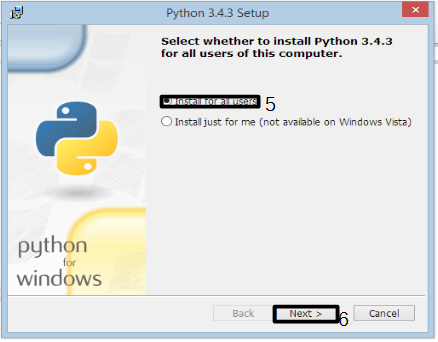
\includegraphics{./manual/images/python-installation-instructions-3.png}
	\caption{How to install python steps 5 and 6}
\end{figure}

\begin{figure}[H]
	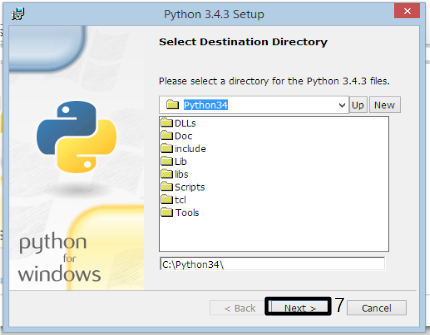
\includegraphics{./manual/images/python-installation-instructions-4.png}
	\caption{How to install python step 7}
\end{figure}

\begin{figure}[H]
	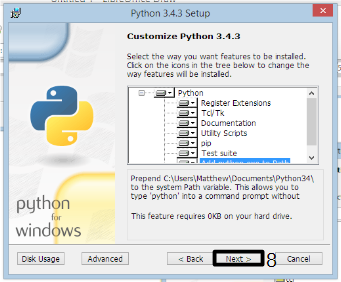
\includegraphics{./manual/images/python-installation-instructions-5.png}
	\caption{How to install python step 8}
\end{figure}

\begin{figure}[H]
	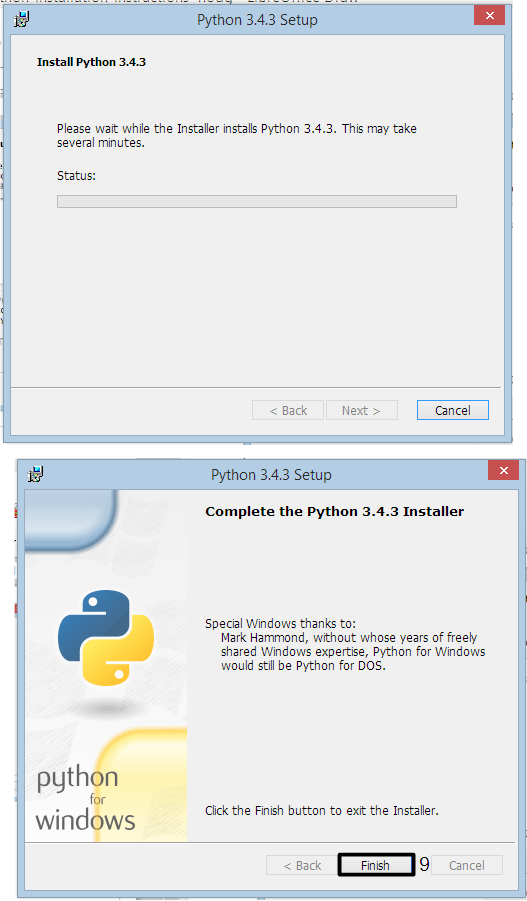
\includegraphics{./manual/images/python-installation-instructions-6.png}
	\caption{How to install python step 9}
\end{figure}
\end{enumerate}

\subsubsection{Installing PyQt}
\begin{enumerate}
	\item go to http://www.riverbankcomputing.co.uk/software/pyqt/download
	\item download the right PyQt .exe file for your system

\begin{figure}[H]
	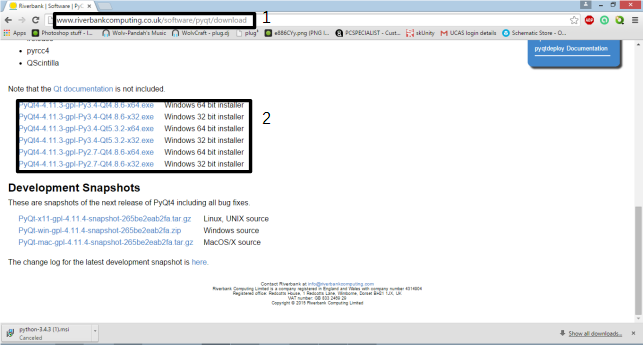
\includegraphics{./manual/images/pyqt-installation-instructions-1.png}
	\caption{How to install python steps 1 and 2}
\end{figure}

	\item navigate to the location of the downloaded .exe file
	
\begin{figure}[H]
	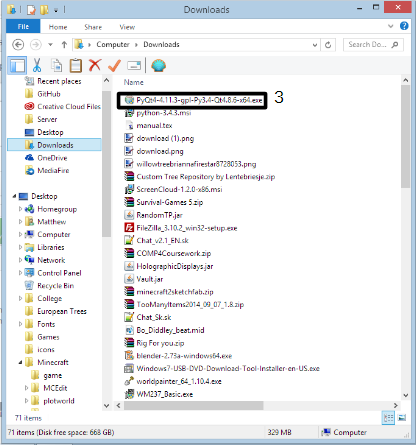
\includegraphics{./manual/images/pyqt-installation-instructions-2.png}
	\caption{How to install python step 3}
\end{figure}

\begin{figure}[H]
	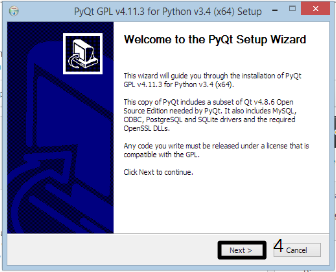
\includegraphics{./manual/images/pyqt-installation-instructions-3.png}
	\caption{How to install python step 4}
\end{figure}

\begin{figure}[H]
	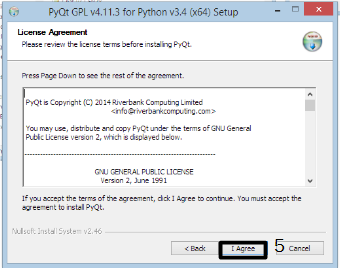
\includegraphics{./manual/images/pyqt-installation-instructions-4.png}
	\caption{How to install python step 5}
\end{figure}

\begin{figure}[H]
	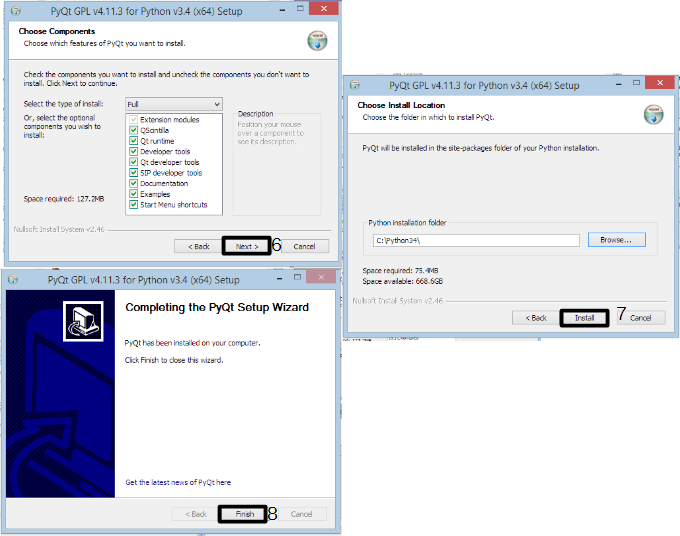
\includegraphics{./manual/images/pyqt-installation-instructions-5.png}
	\caption{How to install python steps 6,7 and 8}
\end{figure}
\end{enumerate}

\subsubsection{Etc.}

\subsection{System Installation}
\label{System_Installation}
\begin{enumerate}
	\item go to https://github.com/MattAnderson16/COMP4Coursework
	\item click the 'Download ZIP' button
	\item navigate to where the downloaded file is saved
	\item open 'COMP4Coursework-master.zip'
	\item open the 'COMP4Coursework-master' folder 
	\item select the 'Implementation' folder
	\item click the 'extract' button
	\item select where you want the folder to be extracted to
	\item click 'OK'
\end{enumerate}

\subsection{Running the System}
\label{Running_the_System}
\begin{enumerate}
	\item navigate to where the system is saved.
	\item open 'new\_main\_window.py'
\end{enumerate}

\section{Tutorial}
\subsection{Introduction}
In this tutorial, I will describe how to use each part of the system effectively under specific questions with screenshots and detailed instructions to walk you through using the system.

\subsection{Assumptions}
This tutorial assumes that you already have Python, PyQt4, MatPlotLib and the main system installed (See the prerequisite installation on page \pageref{Prerequisite_Installation} and the system installation on page \pageref{System_Installation} for instructions on how to install these) and that you can open the system (See Running the System on page \pageref{Running_the_System} for instructions on how to open the system.

\subsection{Tutorial Questions}
\begin{itemize}
	\item How do I add a user?
	\item How do I edit a user?
	\item How do I remove a user?
	\item How do I add a reading?
	\item How do I edit a reading?
	\item How do I remove a reading?
	\item How do I add a cost?
	\item How do I edit a cost?
	\item How do I remove a cost?
	\item How do I add a type?
	\item How do I edit a type?
	\item How do I remove a type?
	\item How do I refresh a table or graph after data has been added, edited or removed?
	\item How do I view a bar chart?
	\item How do I view a pie chart?
	\item How do I view different data on the table?
\end{itemize}

\subsubsection{How do I add a user?}\label{question:add_user}
To add a user, first click the 'profile' option on the main menu and then click the 'new profile' option. From there, type the first name, last name and password of the user you're adding into the text boxes and click the 'confirm' button.
\begin{figure}[H]
	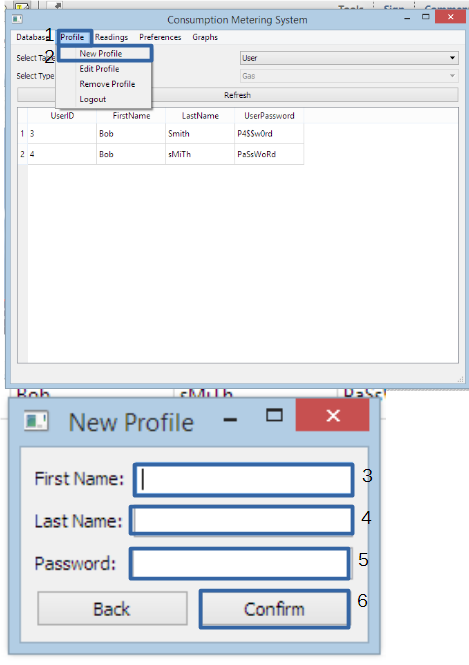
\includegraphics{./manual/images/add_user.png}
	\caption{How to add a user}
\end{figure}

\subsubsection{How do I edit a user?}\label{question:edit_user}
To edit a user, first click the 'profile' option on the main menu and then click the 'edit profile' option. From there, select the user you want to edit and type the new first name, new last name and new password into the text boxes and click the 'confirm' button
\begin{figure}[H]
	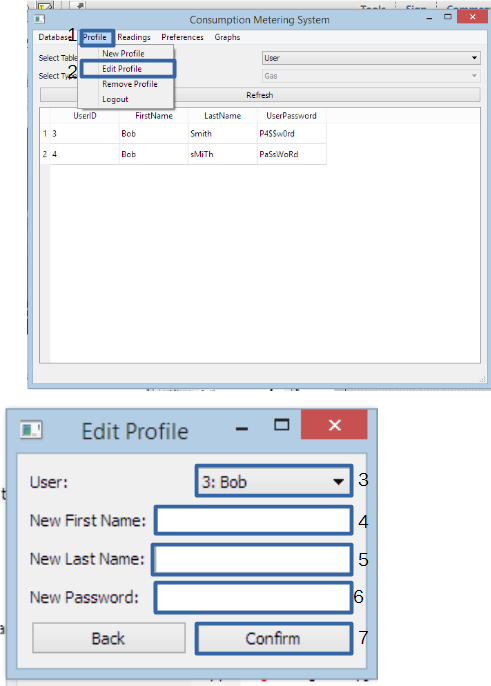
\includegraphics{./manual/images/edit_user.png}
	\caption{How to edit a user}
\end{figure}

\subsubsection{How do I remove a user?}\label{question:remove_user}
To remove a user, first click the 'profile' option on the main menu and then click the 'remove profile' option. From there, select the user you want to remove and click the 'confirm' button.
\begin{figure}[H]
	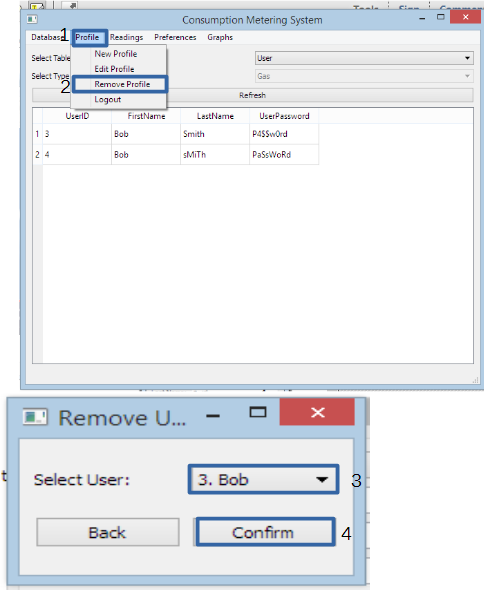
\includegraphics{./manual/images/remove_user.png}
	\caption{How to remove a user}
\end{figure}

\subsubsection{How do I add a reading?}\label{question:add_reading}
\begin{figure}[H]
	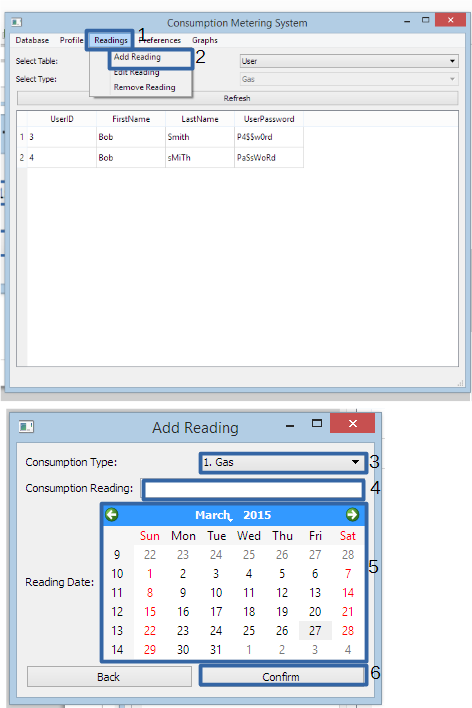
\includegraphics{./manual/images/add_reading.png}
	\caption{How to add a reading}
\end{figure}

\subsubsection{How do I edit a reading?}\label{question:edit_reading}
\begin{figure}[H]
	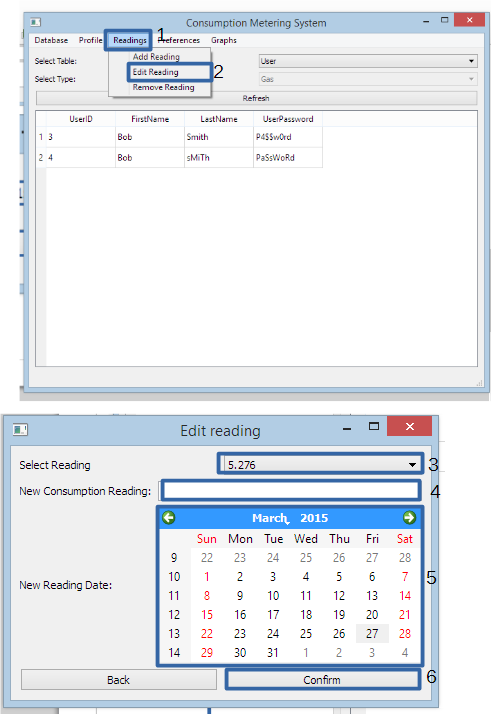
\includegraphics{./manual/images/edit_reading.png}
	\caption{How to edit a reading}
\end{figure}

\subsubsection{How do I remove a reading?}\label{question:remove_reading}
\begin{figure}[H]
	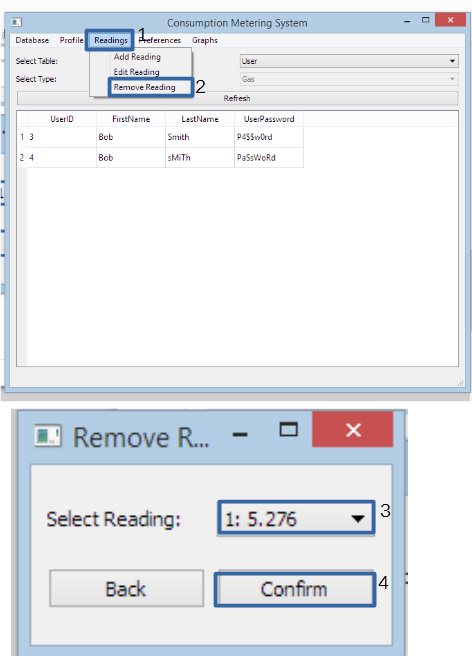
\includegraphics{./manual/images/remove_reading.png}
	\caption{How to remove a reading}
\end{figure}

\subsubsection{How do I add a cost?}\label{question:add_cost}
\begin{figure}[H]
	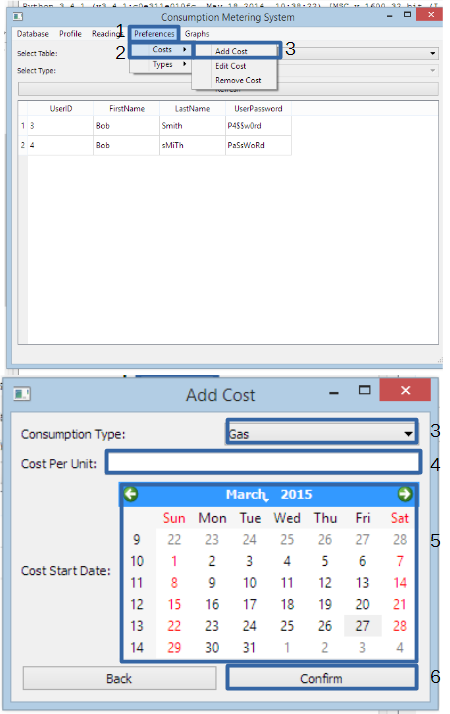
\includegraphics{./manual/images/add_cost.png}
	\caption{How to add a cost}
\end{figure}


\subsubsection{How do I edit a cost?}\label{question:edit_cost}
\begin{figure}[H]
	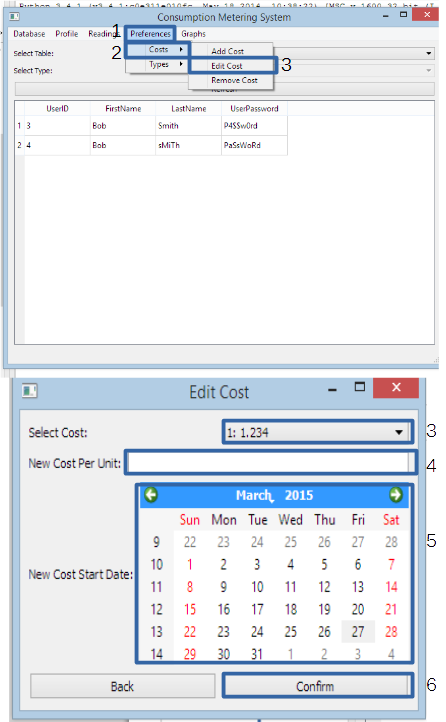
\includegraphics{./manual/images/edit_cost.png}
	\caption{How to edit a cost}
\end{figure}


\subsubsection{How do I remove a cost?}\label{question:remove_cost}
\begin{figure}[H]
	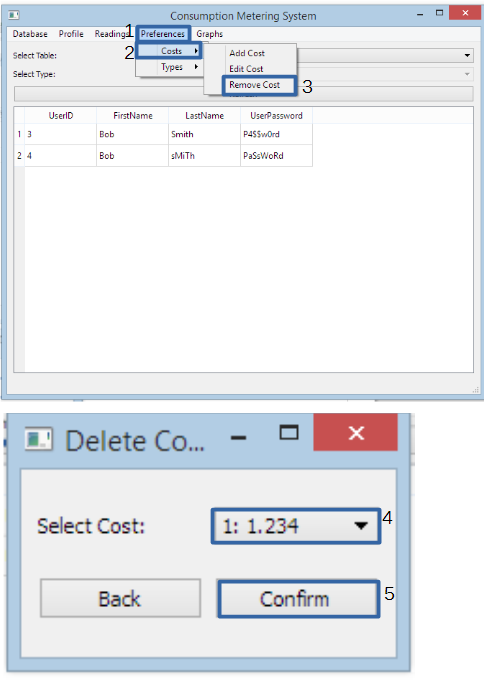
\includegraphics{./manual/images/remove_cost.png}
	\caption{How to remove a cost}
\end{figure}


\subsubsection{How do I add a type?}\label{question:add_type}
\begin{figure}[H]
	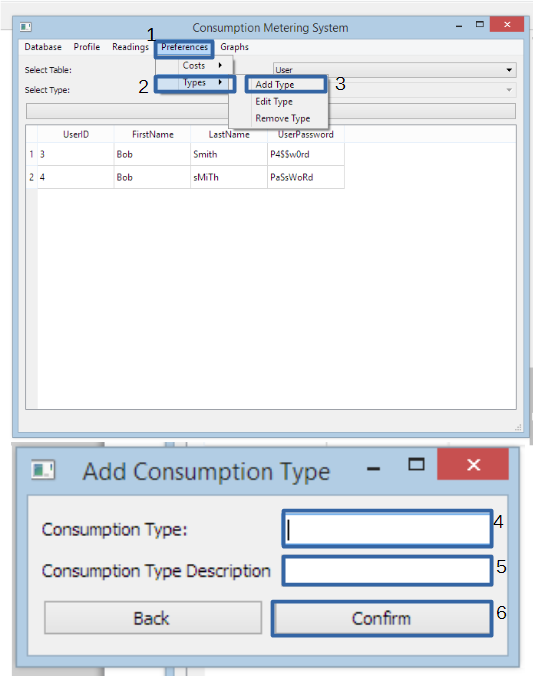
\includegraphics{./manual/images/add_type.png}
	\caption{How to add a type}
\end{figure}

\subsubsection{How do I edit a type?}\label{question:edit_type}
\begin{figure}[H]
	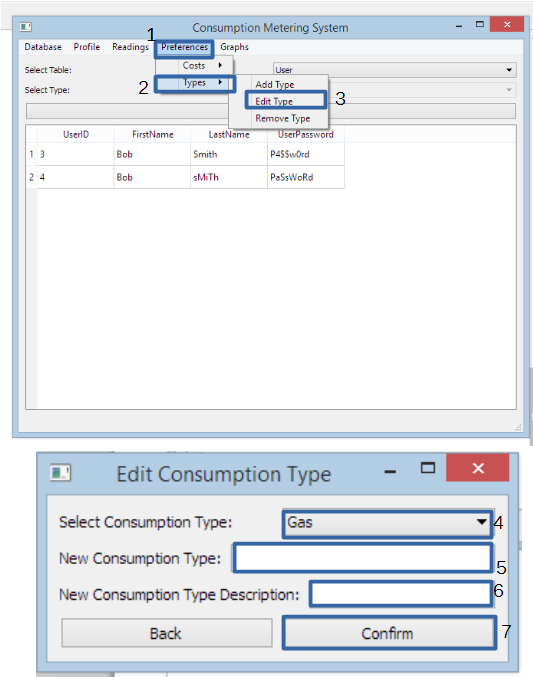
\includegraphics{./manual/images/edit_type.png}
	\caption{How to edit a type}
\end{figure}

\subsubsection{How do I remove a type?}\label{question:remove_type}
\begin{figure}[H]
	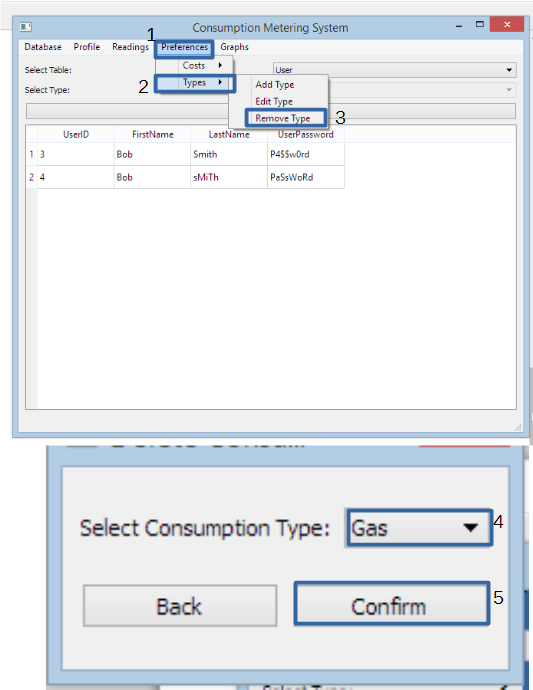
\includegraphics{./manual/images/remove_type.png}
	\caption{How to remove a type}
\end{figure}

\subsubsection{How do I refresh a table or graph after data has been added?}\label{question:refresh_table}
Refreshing a table or graph is as easy as clicking the 'refresh' button above the table.
\begin{figure}[H]
	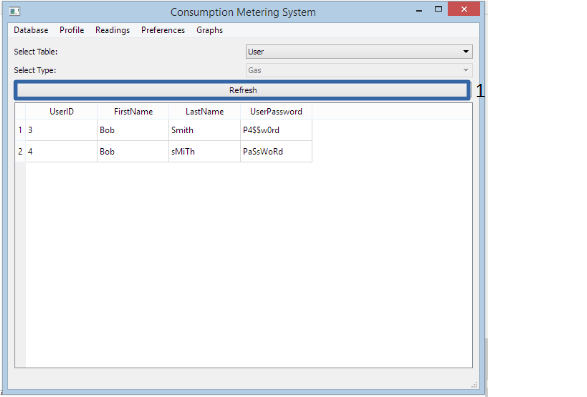
\includegraphics{./manual/images/refresh_table.png}
	\caption{How to refresh a table or graph}
\end{figure}

\subsubsection{How do I view a bar chart?}\label{question:bar_chart}
\begin{figure}[H]
	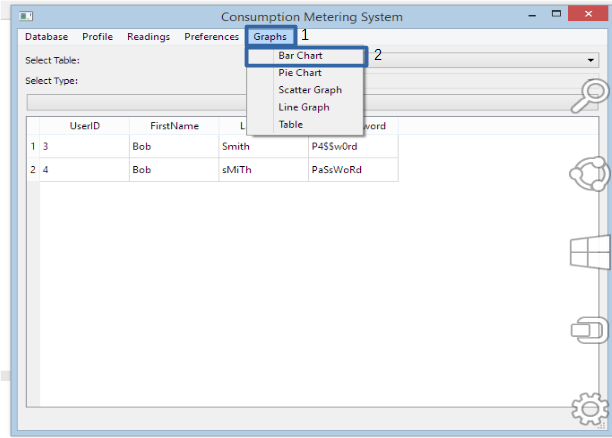
\includegraphics{./manual/images/display_bar_chart.png}
	\caption{How to view a bar chart}
\end{figure}

\subsubsection{How do I view a pie chart?}\label{question:pie_chart}
\begin{figure}[H]
	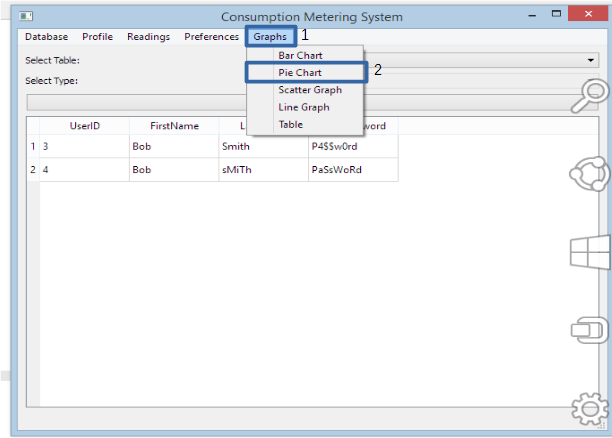
\includegraphics{./manual/images/display_pie_chart.png}
	\caption{How to view a pie chart}
\end{figure}

\subsubsection{How do I view different data on the table?}\label{question:update_table}
\begin{figure}[H]
	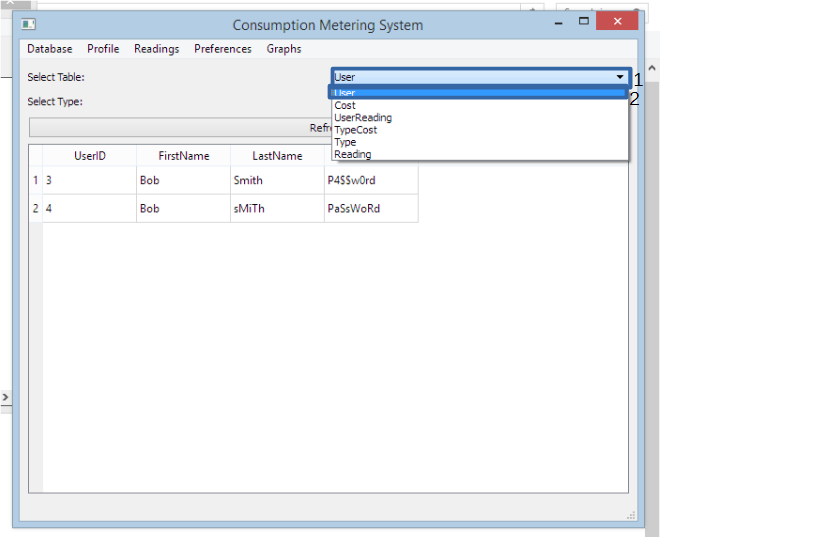
\includegraphics{./manual/images/update_table.png}
	\caption{How to view different data on the table}
\end{figure}

\subsection{Saving}
The system saves data added to the database automatically once the 'confirm' button is pressed after adding, editing or removing data

\subsection{Limitations}
Some limitations of this system are:
\begin{itemize}
	\item It cannot display line or scatter graphs
	\item It cannot change between units
	\item It is not possible to format the database from within the system
	\item It is not possible to change the user for the system
	\item There isn't full validation of data inputs
\end{itemize}

\section{Error Recovery}

\subsection{The system doesn't  reject special characters in the input or editing of first name and/or last name}

\subsubsection{How to recreate this error}
To recreate this error all you need to do is input a first name and/or a last name with special characters into the add or edit user inputs for first name and/or last name.
See questions "How do I add a user?" on page \pageref{question:add_user} or "How do I edit a user?" on page \pageref{question:edit_user} for specific instructructions on how to add and edit user data.

\subsubsection{How to recover from this error}
To recover from this error all you need to do is remove the erroneous user data.
See question "How do I remove a user?" on page \pageref{question:remove_user} for instructions on how to remove user data.

\subsection{The system doesn't display the scatter or line graphs properly}

\subsubsection{How to recreate this error}
To recreate this error you need to try to load the line graph or scatter graph.

\subsubsection{How to recover from this error}
No special actions are needed to recover from this error.

\subsection{The system doesn't display bar charts or pie charts when there is erroneous data}

\subsubsection{How to recreate this error}
To recreate this error you need to add erroneous data to the database and then load the bar chart or pie chart.

\subsubsection{How to recover from this error}
To recover from this error remove any erroneous data and refresh the graph.

\subsection{The system doesn't reject erroneous data from the add reading window}

\subsubsection{How to recreate this error}
To recreate this error add erroneous data to the database.
See question `How do I add reading data?'' on page \pageref{question:add_reading} on how to add reading data.

\subsubsection{How to recover from this error}
To recover from this error remove the erroneous data.
See question `How do I remove reading data?'' on page \pageref{question:remove_reading} on how to remove data.

\section{System Recovery}

\subsection{Backing-up Data}
\begin{enumerate}
	\item right click the database file and copy it
\begin{figure}[H]
	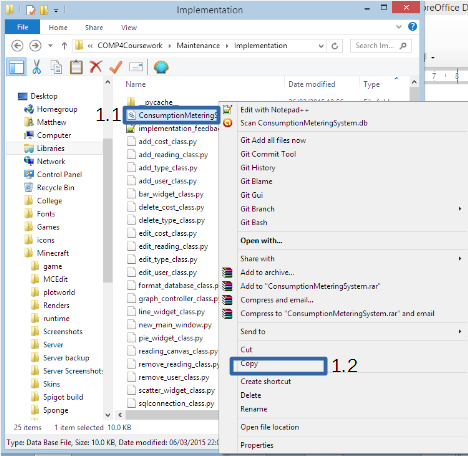
\includegraphics{./manual/images/backup-step-1.png}
\end{figure}
	\item navigate to the backup folder
	\item paste the database in the backup folder
\begin{figure}[H]
	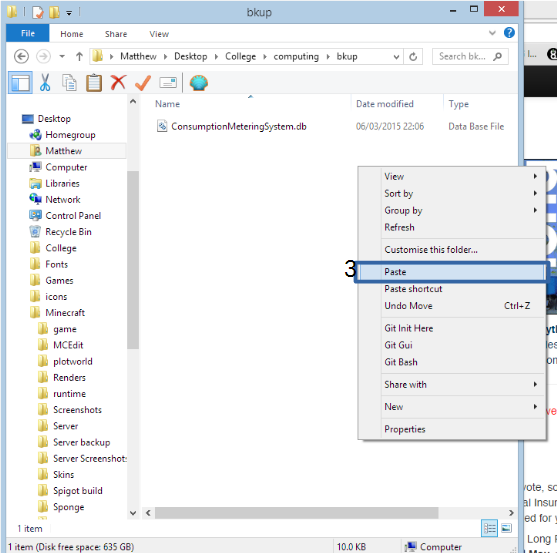
\includegraphics{./manual/images/backup-step-3.png}
\end{figure}
\end{enumerate}
\subsection{Restoring Data}
\begin{enumerate}
	\item right click the database file and copy it
\begin{figure}[H]
	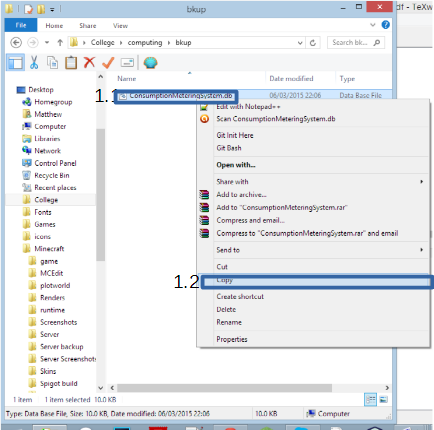
\includegraphics{./manual/images/restore-step-1.png}
\end{figure}
	\item navigate to the system folder
	\item paste the database in the system folder
\begin{figure}[H]
	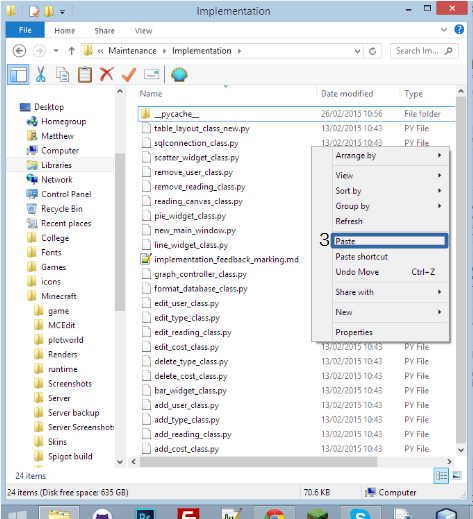
\includegraphics{./manual/images/restore-step-3.png}
\end{figure}
\end{enumerate}

\stopcontents[chapters]